
\unsubsection{Función reciproca}
La función reciproca se define como:
\begin{equation}
    w=\frac{1}{z}
\end{equation}
Esta es una transformación no lineal.
Plantemos una circunferencia genérica centrada en el origen:
\begin{equation}
\begin{aligned}
    &z_a=re^{j\theta}\begin{cases}
        r=\kappa\\
        -\pi<\theta\leq\pi
    \end{cases}
\end{aligned}
\end{equation}
Aplicándole la transformación obtenemos:
\begin{equation}
\begin{aligned}
     w_a=\frac{1}{z_a}\lrah &w_a=\frac{1}{re^{j\theta}}\lrah w_a=\frac{1}{r}e^{-j\theta}\begin{cases}
        r=\kappa\\
        -\pi<\theta\leq\pi
        \end{cases}
\end{aligned}
\end{equation}
Planteamos un cambio de variable:
\begin{equation}
\begin{aligned}
    \phi=-\theta \lrah -\pi<\theta\leq\pi&\\
                        -\pi<-\phi\leq\pi&\\
                        \pi>\phi\geq-\pi&
\end{aligned}
\end{equation}
Como vemos el argumento sigue existiendo en un intervalo de modulo $2\pi$, esto quiere decir que una función reciproca solo modifica el radio de la circunferencia. El radio $\kappa$ de una circunferencia en el plano complejo $z$ pasaría a ser de radio $\frac{1}{\kappa}$ en el plno complejo $w$. Se pueden denotar 3 casos distintos:
\begin{equation}
    \begin{cases}
        \kappa=1 \lrah \frac{1}{\kappa}=1\\
        \kappa\leq 1 \lrah \frac{1}{\kappa}\geq1\\
        \kappa\geq 1 \lrah \frac{1}{\kappa}\leq1
    \end{cases}
\end{equation}
Entonces a mayor radio en el plano $z$ menor sera el radio en $w$ siendo una circunferencia de radio uno el limite entre estas distintas regiones en el comportamiento.
\begin{figure}[H]
\centering
    \begin{minipage}{0.4\textwidth}
    \centering
       \begin{tikzpicture}[scale=0.7]
    \draw[thin,gray!40] (-4,-4) grid (4,4);
    \draw[<->] (-4,0)--(4,0) node[right] {$R$};
    \draw[<->] (0,-4)--(0,4) node[above]{$j$};
    \fill[fill=mlgb, fill opacity=0.6,even odd rule] (-4, -4) rectangle (4,4)(0, 0) circle (2);
    \draw [black,line width=2pt,fill=vorange,fill opacity=0.6](0, 0) circle (2);
    \draw[line width=1pt,|-|] (0,0) -- (2,0) node[midway,above,sloped]{$r=1$};
\end{tikzpicture}
\caption*{Regiones en el plano $z$}
    \label{fig:InvF1}
    \end{minipage}
    
   \begin{minipage}{0.4\textwidth}
    \centering
       \begin{tikzpicture}[scale=0.7]
    \draw[thin,gray!40] (-4,-4) grid (4,4);
    \draw[<->] (-4,0)--(4,0) node[right] {$R'$};
    \draw[<->] (0,-4)--(0,4) node[above]{$j'$};
    \path[fill=vorange, fill opacity=0.6,even odd rule] (-4, -4) rectangle (4,4) (0,0) circle (2);
    \draw [line width=2pt,black,fill=mlgb,fill opacity=0.6](0, 0) circle (2);
    \draw[line width=1pt,|-|] (0,0) -- (2,0) node[midway,above,sloped]{$r=1$};
\end{tikzpicture}
\caption*{Regiones en el plano $w$}
    \label{fig:InvF2}
    \end{minipage}
    \caption{}
    \label{fig:InvF}
\end{figure}
Esto se puede interpreta como que la función reciproca toma los puntos interiores del circulo unitario y los mapea en puntos exteriores al circulo unitario en el plano $w$ y viceversa.

Plantemos ahora una linea vertical, para ver como la función reciproca modifica la malla del plano $z$:
\begin{equation}
    z_a=\kappa+jy
\end{equation}
$\kappa$ siendo una constante.

Aplicándole la función reciproca se obtiene:
\begin{equation}
\begin{aligned}
      w_a=\frac{1}{z_a}\lrah w_a&=\frac{1}{\kappa+jy}\\
                             w_a&=\frac{1}{\kappa+jy}\cdot\frac{\kappa-jy}{\kappa-jy}\\
                              w_a&=\frac{\kappa-jy}{\kappa^2+y^2}\\
                               (u+jv)&=\underbrace{\frac{\kappa}{\kappa^2+y^2}}_\text{\clap{u~}}-j\underbrace{\frac{y}{\kappa^2+y^2}}_\text{\clap{v~}}\\
\end{aligned}
\end{equation}
Recordemos que la variable $w=u+jv$ entonces el mapeo de la recta estará dado por el sistema de ecuaciones:
\begin{equation}
    \begin{cases}
        u=\frac{\kappa}{\kappa^2+y^2}\\
        v=-\frac{y}{\kappa^2+y^2}
    \end{cases}
\end{equation}
Ambas ecuaciones son muy similares entre si, solo difieren en el numerador esto nos permite realizar un paso intermedio simple. Podes expresar $u$ en función de $v$ e $y$ para poder despejar la variable $y$.Luego aplicamos el método de sustitución y así eliminaremos una de nuestras variables dejando una función de 2 variables independientes. 
Vemos que:
\begin{equation}
     u=-\frac{v\kappa}{y} \lrah y=-\frac{v\kappa}{u}
\end{equation}
Resolviendo por sustitución en la ecuación $u=...$ :
\begin{equation}
    \begin{aligned}
        u=\frac{\kappa}{\kappa^2+y^2}\lrah &u=\frac{\kappa}{\kappa^2+(\cfrac{v\kappa}{u})^2}\lrah u=\frac{\kappa}{\kappa^2+\cfrac{v^2\kappa^2}{u^2}}\\
        &u=\frac{\bcancel{\kappa}}{\kappa^{\bcancel{2}}(1+\cfrac{v^2}{u^2})}\lrah u(1+\cfrac{v^2}{u^2})=\frac{1}{\kappa}\\
        &u+\cfrac{v^2}{u}=\cfrac{1}{\kappa}\lrah -v^2=(u-\cfrac{1}{\kappa})\cdot(u)\\
        &0=(u^2-\cfrac{u}{\kappa})+v^2\lrah\cfrac{1}{4\kappa^2}=(u^2-\cfrac{u}{\kappa}+\cfrac{1}{4\kappa^2})+v^2\\
        &(\cfrac{1}{2\kappa})^2=(u-\cfrac{1}{2\kappa})^2+v^2\\
        \label{eq:1/ZVer}
    \end{aligned}
\end{equation}
 Si recordamos la ecuación que describe una circunferencia en el plano de 2 dimensiones reales vemos que son prácticamente idénticas:
 \begin{equation}
     r^2=(x-x_0)^2+(y-y_0)^2
 \end{equation}
 Entones podemos afirmar que cualquier linea vertical desplazada en $\kappa$ sera mapeada en una circunferencia con centro $\frac{1}{2\kappa}$ sobre el eje real y de radio igual a su desplazamiento $r=\frac{1}{2\kappa}$. Al ser el modulo del radio igual al modulo del desplazamiento todas las circunferencias pasaran por el punto$(0,j0)$. 
\begin{figure}[H]
\centering
    \begin{minipage}{0.4\textwidth}
    \centering
       \input{Plots/FuncionesComplejos/Mappeo/Invers/InvF3}
    \end{minipage}
   \begin{minipage}{0.41\textwidth}
    \centering
       \begin{tikzpicture}
    \coordinate (a) at (1,0);
    \draw[thin,gray!40] (-2,-2) grid (2,2);
    
    \path[fill=mlgb, fill opacity=0.6,even odd rule] (0, -2) rectangle (2,2) (a) circle (1);
    \path [line width=2pt,black,fill=vorange,fill opacity=0.6](a) circle (1);
    
    \draw[<->] (-2,0)--(2,0) node[right] {$R$};
    \draw[<->] (0,-2)--(0,2) node[above]{$j$};
    
    
    \draw[line width=2pt] (1,0) circle(1);
    \draw[fill=black] (a) circle(2pt) node[below]{$\frac{1}{2\kappa}$};
    \draw[line width=1pt,black,|-|] (0,0)--(a) node[midway,above,sloped]{$\frac{1}{2\kappa}$};
\end{tikzpicture}
\caption*{Mapeo linea vertical}
    \end{minipage}
    \caption{}
    \label{fig:InvFV1}
\end{figure}
El mapeo para lineas horizontales es similar.
\begin{figure}[H]
\centering
    \begin{minipage}{0.4\textwidth}
    \centering
       \begin{tikzpicture}

    \draw[thin,gray!40] (-2,-2) grid (2,2);

    \path[draw=gray!40, fill=mlgb, fill opacity=0.6] (-2,1) -- (2,1) -- (2,0) -- (-2,0);
    \path[draw=gray!40, fill=vorange, fill opacity=0.6] (-2,1) -- (2,1) -- (2,2) -- (-2,2);
    
    \draw[<->] (-2,0)--(2,0) node[right] {$R$};
    \draw[<->] (0,-2)--(0,2) node[above]{$j$};
    
    \draw[fill=black] (0,1) circle(2pt) node[anchor=south east]{$\kappa$};
    \draw[line width=2pt,black,stealth-stealth] (-2,1)--(2,1) node[anchor=south west]{$(\kappa,jt)$};
\end{tikzpicture}
\caption*{Linea Horizontal}
    \end{minipage}
   \begin{minipage}{0.41\textwidth}
    \centering
       \input{Plots/FuncionesComplejos/Mappeo/Invers/InvF7}
    \end{minipage}
    \caption{}
    \label{fig:InvFV2}
\end{figure}
 Analizando la ecuación que rige el centro de la circunferencia vemos que a mayor distancia del la ordenada al origen en el plano $z$ menor va hacer su distancia a la ordenada al origen en el plano $w$ y menor va a ser su radio. Esto lo podemos relacionar con como, la función inversa, mapea a una circunferencia, ya que si en el plano $z$ la linea pasa por un punto $\kappa$ cercano a $0$ esta sera mapeada en una circunferencia de radio cercano a infinito, comportamiento que valida la idea que la función inversa mapea los puntos dentro de la circunferencia unitria fuera de este en el plano $w$. De todas maneras parte de los punto de la recta se siguen mapeando dentro de la circunferencia unitaria entonces la función reciproca más bien toma el plano $z$ y lo curva sobre la ordenada al origen en el infinito.
 \begin{figure}[H]
     \centering
     \begin{tikzpicture}
    \draw [thin,mlgb] (-6,-6) grid (6,6);
    \draw[mlgb,<->] (-6,0)--(6,0) node[anchor= north west] {$R$};
    \draw[mlgb,<->] (0,-6)--(0,6) node[anchor=south east]{$j$};
    \draw[<->] (-6,0)--(6,0) node[anchor=south west] {$R'$};
    \draw[<->] (0,6)--(0,-6) node[anchor=south west]{$j'$};
    \clip (-6,-6) rectangle (6,6);
    \foreach \c in {0.5,1,...,4.5} {
        \draw[line width=0.75pt,gray] (\c,0) circle(\c);
    }
    \foreach \c in {0.5,1,...,4.5} {
        \draw[line width=0.75pt,gray] (-\c,0) circle(\c);
    }
    \foreach \c in {0.5,1,...,4.5} {
        \draw[line width=0.75pt,gray] (0,\c) circle(\c);
    }
    \foreach \c in {0.5,1,...,4.5} {
        \draw[line width=0.75pt,gray] (0,-\c) circle(\c);
    }
    %\foreach \c in {1,2...,7} {
    %    \draw[line width=1pt,gray!40] (0,(1/(2\c))) circle((1/(2\c))^2);
    %}
    % \draw[line width=1pt] (0,0) circle(2);
    % \draw[line width=0.5pt,mlgb,dashed] (0,0) circle(2);
    % \draw[line width=0.5pt,blue,dashed] (0,0) circle(1);
    % \draw[line width=0.5pt,vorange,dashed] (0,0) circle(6);
    % \draw[line width=1pt,blue] (0,0) circle(4);
    % \draw[line width=1pt,vorange] (0,0) circle(0.6666);
    
    
\end{tikzpicture}
\caption{Plano $w$ graficado sobre el plano $z$ siendo $f_{z}$ un función reciproca}
 \end{figure}

En el caso del punto $(0,j0)$ la función reciproca es igual a $\infty$.

\unsubsection{Función potencia}
La función potencia se define como:
\begin{equation}
    w=z^n
\end{equation}
\unsubsubsection{Función $z^2$}
Planteando una circunferencia/arco genérico y una segmento de recta que pase por el punto $(0,j0)$:
\begin{equation}
    \begin{aligned}
        &z_a=re^{j\theta}\begin{cases}
            r=\kappa\\
            a\leq\theta\leq b
        \end{cases}\\
        \\
        &z_b=re^{j\theta}\begin{cases}
            c\leq r\leq d\\
            \theta=\kappa
        \end{cases}
    \end{aligned}
\end{equation}
Aplicándoles la función:
\begin{equation}
    w=z^2
\end{equation}
Obtenemos:
\begin{equation}
    \begin{aligned}
        &w_a={z_a}^2\lrah w_a=r^2e^{2j\theta}\begin{cases}
            r=\kappa\\
            a\leq\theta\leq b
        \end{cases}\\
        \\
        &w_b=z_b^2\lrah w_b=r^2e^{2j\theta}\begin{cases}
            a\leq r\leq\ b\\
            \theta=\kappa
        \end{cases}
    \end{aligned}
\end{equation}
Realizando cambios de variable $\phi=2\theta$ y $r'=r^2$ respectivamente:
\begin{equation}
\begin{cases}
    w_a=r^2e^{j\phi}\begin{cases}
            r=\kappa\\
            2a\leq\phi\leq 2b
        \end{cases}\\
    \\
    w_b=r'e^{2j\theta}\begin{cases}
        (a)^2\leq r'\leq\ b^2\\
        \theta=\kappa
        \end{cases}
\end{cases}
\end{equation}
Vemos que en el caso del arco $z_a$, la función $z^2$ extendió el rango de valores que podía tomar el argumento además de amplificar su radio. Si tuviéramos un circulo completo los limites del intervalo del argumento sobre pasarían el intervalo limite de $-\pi<\theta\leq\pi$. Podemos decir entonces que con un arco en $z$ podemos definir una circunferencia en el plano $w$. Esto lo podemos pensar como una dilatación del plano $z$, descripta en la figura \ref{fig:z^2F1}.

Y en el caso de la segmento de recta, se roto su argumento en $\theta$ y el intervalo de valores que pude tomar $r'$ son solo número4s reales positivos. Analizando los dominios, en el plno 
$z$ y $w$ de los módulos de semirrectas y segmentos:
\begin{equation}
    \begin{cases}
        0\leq r\leq\infty\lrah 0\leq r'\leq\infty\\
        -1\leq r\leq\ 2\lrah 1\leq r'\leq\ 4\\
        -3\leq r\leq\ 1\lrah 9\leq r'\leq\ 1\\
    \end{cases}
\end{equation}
Entonces podemos decir que la función $z^2$ mapea segmentos y semirrectas que no estén desplazadas en el plano $z$ en otros segmentos y semirrectas que posen un argumento de $2j\theta$. 


En el caso de la recta obtenemos un conflicto en el intervalo:
\begin{equation}
    \begin{cases}
        -\infty\leq r\leq\infty\lrah\infty\leq r'\leq\infty\\
    \end{cases}
\end{equation}
Para solucionar esta contradicción se puede construir una recta a partir de 2 semirrectas de modulo $0\leq r\leq\infty$ y de argumentos $j(\theta)$ y $j(\theta+\pi)$ para representar la parte positiva y negativa respectivamente. Aplicando la transformación vemos que los módulos de ambas semi rectas son iguales y los argumentos también. Recordando que $+2\pi$ en la expresión de un argumento equivale a una rotación de $360^{\circ}$:
\begin{equation}
    \begin{cases}
        j\theta\lrah j2\theta\\
        j(\theta+\pi)\lrah j(2\theta+2\pi)=j2\theta
    \end{cases}
\end{equation}
Una recta entonces se mapea en 2 semirrectas identicas.

\begin{figure}[H]
    \centering
    \begin{minipage} {0.49\textwidth}
    \centering
        \begin{tikzpicture}[scale=0.7]
    
    \foreach \ang in {0,...,31} {
        \draw [gray!40] (0,0) -- (\ang * 180 / 16:4);
    }
    \foreach \s in {0,0.5,...,3.5} {
        \draw [gray!40] (0,0) circle (\s);
    }
    \path[fill=mlgb, fill opacity=0.6] (0,0)--(4,0) arc(0:90:4) --(0,0);
    \path[fill=vorange, fill opacity=0.6] (0,0)--(4,0) arc(360:270:4)--(0,0);
    
    \draw[<->] (-4,0)--(4,0) node[right] {$R$};
    \draw[<->] (0,-4)--(0,4) node[above]{$j$};
    \draw [black,line width=0.5pt] circle (4);
    \draw[line width=0.75pt,mdrd,|-|] (0.3827*0.5,0.9239*0.5) arc (67.5:112.5:0.5);
    \draw[line width=0.75pt,mdblu,|-|] (0.3827,-0.9239) arc (-67.5:-112.5:1);
    \draw[line width=0.75pt,mblk,|-|] (-0.1951*1.5,0.9808*1.5) arc (101.25:168.75:1.5);
    
   % \path[fill opacity=0.6,pattern=dots,pattern color=mdblu, even odd rule] (0,0)--(0,4) arc(90:180:4)--(0,0);
   % \path[fill opacity=0.6,pattern=dots,pattern color=mdrd, even odd rule] (0,0)--(0,-4) arc(270:180:4)--(0,0);
\end{tikzpicture}
\caption*{Plano $z$}

    \end{minipage}
    \begin{minipage} {0.49\textwidth}
    \centering
        \begin{tikzpicture}[scale=0.7]
    \foreach \ang in {0,...,31} {
        \draw [gray!40] (0,0) -- (\ang * 360 / 16:4);
    }
    \foreach \s in {0.25,1,2.25,4} {
        \draw [gray!40] (0,0) circle (\s);
    }
    \path[fill=mlgb, fill opacity=0.6] (0,0)--(4,0) arc(0:180:4) --(0,0);
    \path[fill=vorange, fill opacity=0.6] (0,0)--(4,0) arc(360:180:4)--(0,0);
    
    \draw[<->] (-4,0)--(4,0) node[right] {$R$};
    \draw[<->] (0,-4)--(0,4) node[above]{$j$};
    \draw [black,line width=0.6pt] circle (4);
    \draw[line width=0.75pt,mblk,|-|] (-0.9239*2.25,-0.3827*2.25) arc (202.5:337.5:2.25);
    
    
    \draw[line width=0.75pt,mdrd,|-|] (-0.70711*0.25,0.70711*0.25) arc (135:225:0.25);
    \draw[line width=0.75pt,mdblu,|-|] (-0.70711,-0.70711) arc (-135:-225:1);

    
    %\path[fill opacity=0.6,pattern=dots,pattern color=mdblu,even odd rule] (0,0)--(4,0) arc(360:180:4)--(0,0);
    %\path[fill opacity=0.6,pattern=dots,pattern color=mdrd, even odd rule] (0,0)--(0,-4) (0,0)--(4,0) arc(0:180:4) --(0,0);
\end{tikzpicture}
\caption*{Plano $w$}

    \end{minipage}
    \caption{}
    \label{fig:z^2F1}
\end{figure}

Ahora que tenemos una idea de como afecta el plano complejo la función $z^2$, plantemos una recta vertical y horizontal para terminar de comprender como se modifica el espacio.
\begin{equation}
    \begin{cases}
        z_a=\kappa+jy\\
        z_b=x+j\kappa
    \end{cases}
\end{equation}
Aplicando la función $z^2$ a $z_a$:
\begin{equation}
    w_a={z_a}^2\lrah u+jv=\kappa^2-y^2+2jy\kappa
    \begin{cases}
        u=\kappa^2-y^2\\
        v=2y\kappa
    \end{cases}
\end{equation}
De la ecuación que describe $v$ podemos depejar la variable $y$ para luego resolver por sustitución.
\begin{equation}
    v=2y\kappa\lrah y=\frac{v}{2\kappa}
\end{equation}
\begin{equation}
\begin{aligned}
     u=\kappa^2-y^2\lrah &u=\kappa^2-(\frac{v}{2\kappa})^2\\
                        &(u-\kappa^2)=-\frac{v^2}{4\kappa^2}\\
                        \\
                        &(u-\kappa^2)4\kappa^2=-v^2
\end{aligned}
\end{equation}
Entonces una recta vertical centrada en $\kappa$ se mapea en una parábola de vértice $(\kappa^2,j0)$ y foco $\kappa^2$. Esto conlleva a que cualquier recta vertical se mapea en una parábola horizontal que abré hacia la izquierda y siempre tiene un vértice sobre el eje real positivo.
\begin{figure}[H]
    \centering
    \begin{minipage}{0.49\textwidth}
    \centering
        \begin{tikzpicture}
    \draw[thin,gray!40] (-3,-3) grid (3,3);
    \fill[fill=vorange, fill opacity=0.6,even odd rule] (-3,-3) rectangle (3,3) (1,-3) rectangle (2,3);
    \fill[fill=mlgb, fill opacity=0.6] (1,-3) rectangle (2,3);
    \draw[<->] (-3,0)--(3,0) node[right] {$R$};
    \draw[<->] (0,-3)--(0,3) node[above]{$j$};
    
    \draw[line width=2pt,black,stealth-stealth] (1,-3)--(1,3) node[midway, above left]{$\kappa_1$};
    \draw[line width=2pt,black,stealth-stealth] (2,-3)--(2,3) node[midway, above right]{$\kappa_2$};
\end{tikzpicture}
\caption*{Lineas verticales}
    \end{minipage}
    \begin{minipage}{0.49\textwidth}
    \centering
        \begin{tikzpicture}
        \draw[thin,gray!40] (-3,-3) grid (3,3);
        \path[rotate=90,opacity=0.6,fill=vorange,even odd rule] (-3,-3) rectangle (3,3) plot[smooth,domain=-2.55:2.55] (\x, {((\x)^2/1.3)-2}) plot[smooth,domain=-1.4142:1.4142] (\x, {((\x)^2*2)-1});
        \path[rotate=90,line width=2pt,fill=mlgb,fill opacity=0.6,even odd rule] plot[smooth,domain=-2.55:2.55] (\x, {((\x)^2/1.3)-2}) plot[smooth,domain=-1.4142:1.4142] (\x, {((\x)^2*2)-1});
        \draw[<->] (-3,0)--(3,0) node[right] {$R$};
        \draw[<->] (0,-3)--(0,3) node[above]{$j$};
        \draw[rotate=90,line width=2pt]   plot[smooth,domain=-2.55:2.55] (\x, {((\x)^2/1.3)-2}) (0,-2) node[above right]{$\kappa_2'$} plot[smooth,domain=-1.4142:1.4142] (\x, {((\x)^2*2)-1}) (0,-1) node[left]{$\kappa_1'$};
\end{tikzpicture}
\caption*{Plano complejo $w$}
    \end{minipage}
    \caption{}
    \label{fig:Z^2VF}
\end{figure}
Realizando el mismo procedimiento para las lineas horizontales obtenemos la ecuación:
\begin{equation}
    (u+\kappa^2)4\kappa^2=v^2
\end{equation}
A diferencia del mapeo para rectas verticales, el mapeo de rectas horizontales de como resultado parábolas horizontales que abren hacia la derecha y posen un vértice sobre el eje real negativo.
\begin{figure}[H]
    \centering
    \begin{minipage}{0.49\textwidth}
    \centering
        \begin{tikzpicture}
    \draw[thin,gray!40] (-3,-3) grid (3,3);
    \fill[fill=vorange, fill opacity=0.6,even odd rule] (-3,-3) rectangle (3,3) (-3,1) rectangle (3,2);
    \fill[fill=mlgb, fill opacity=0.6] (-3,1) rectangle (3,2);
    \draw[<->] (-3,0)--(3,0) node[right] {$R$};
    \draw[<->] (0,-3)--(0,3) node[above]{$j$};
    
    \draw[line width=2pt,black,stealth-stealth] (-3,1)--(3,1) node[midway, below right]{$\kappa_1$};
    \draw[line width=2pt,black,stealth-stealth] (-3,2)--(3,2) node[midway, above right]{$\kappa_2$};
\end{tikzpicture}
\caption*{Lineas horizontales}
    \end{minipage}
    \begin{minipage}{0.49\textwidth}
    \centering
        \input{Plots/FuncionesComplejos/Mappeo/Z^2/Z^2HF2}
    \end{minipage}
    \caption{}
    \label{fig:Z^2HF}
\end{figure}
Cabe aclarar que lo mostrado en las figuras \ref{fig:Z^2VF} y \ref{fig:Z^2HF} solo son una representación valida para cuando $\kappa_1$ y $\kappa_2$ son mayor a $1$. Si este no fuera el caso, se invertirían las posiciones relativas de $\kappa_1'$ y $\kappa_2'$.
\begin{figure}[H]
    \centering
    \begin{tikzpicture}
    \draw [thin,mlgb] (-6,-6) grid (6,6);
    \draw[mlgb,<->] (-6,0)--(6,0) node[anchor= south west] {$R$};
    \draw[mlgb,<->] (0,-6)--(0,6) node[anchor=south east]{$j$};
    \draw[<->] (0,0)--(6,0) node[anchor= north west] {$R'$};
    \draw[<->] (0,0)--(-6,0) node[anchor=south east]{$j'$};

    \foreach \c in {0.2,0.4,...,1} {
        \draw [rotate=90,gray] plot[smooth,domain=-(sqrt((6+\c^2)*(4*\c^2))):(sqrt((6+\c^2)*(4*\c^2)))](\x, {((\x)^2/(4*\c^2))-\c^2});
    }
    \foreach \c in {1.2,1.4,...,2.4} {
        \draw [rotate=90,gray] plot[smooth,domain=-6:6](\x, {((\x)^2/(4*\c^2))-\c^2});
    }

   \foreach \c in {0.2,0.4,...,1} {
        \draw [rotate=-90,gray] plot[smooth,domain=-(sqrt((6+\c^2)*(4*\c^2))):(sqrt((6+\c^2)*(4*\c^2)))](\x, {((\x)^2/(4*\c^2))-\c^2});
    }
    \foreach \c in {1.2,1.4,...,2.4} {
        \draw [rotate=-90,gray] plot[smooth,domain=-6:6](\x, {((\x)^2/(4*\c^2))-\c^2});
    }
\end{tikzpicture}
\caption{Plano $w$ graficado sobre el plano $z$ siendo $f_{z}$ un función $z^2$}
    \label{fig:Z^2FC}
\end{figure}
\unsubsubsection{Función $z^{1/2}$}
La función $z^{1/2}$ al ser la inversa de la función $z^2$ genera el efecto contrario, contrayendo el espacio $z$, en su totalidad, en los cuadrantes $1$ y $4$ en el plano $w$.
Planteando una arco/circunferencia genérica que tengan por centro el punto $(0,j0)$ y una recta que pase por ese mismo, vemos que sus mapeos respectivos son entonces:
\begin{equation}
    \begin{aligned}
        &w_a={z_a}^{\cfrac{1}{2}}\lrah w_a=\sqrt{r}e^{j\frac{\theta}{2}}\begin{cases}
            r=\kappa\\
            -a\leq\theta\leq b
        \end{cases}\\
        \\
        &w_b=z_b^{\cfrac{1}{2}}\lrah w_b=\sqrt{r}e^{j\frac{\theta}{2}}\begin{cases}
            a\leq r\leq\ b\\
            \theta=\kappa
        \end{cases}
    \end{aligned}
\end{equation}
Realizando cambios de variable $\phi=\frac{\theta}{2}$ y $r'=\sqrt{r}$ respectivamente:
\begin{equation}
\begin{cases}
    w_a=\sqrt{r}e^{j\phi}\begin{cases}
            r=\kappa\\
            -\frac{a}{2}\leq\phi\leq \frac{b}{2}
        \end{cases}\\
    \\
    w_b=r'e^{j\frac{\theta}{2}}\begin{cases}
        \sqrt{a}\leq r'\leq\ \sqrt{b}\\
        \theta=\kappa
        \end{cases}
\end{cases}
\end{equation}
Se pude apreciar como se reduce el tamaño del intervalo para las variables independientes. Esto se puede interpretar como una contracción del espacio, expresado en la figura \ref{fig:z^0.5F1}.
\begin{figure}[H]
    \centering
    \begin{minipage}{0.49\textwidth}
    \centering
        \input{Plots/FuncionesComplejos/Mappeo/z^0.5/z^0.5F1}
    \end{minipage}
    \begin{minipage}{0.49\textwidth}
    \centering
        \begin{tikzpicture}[scale=0.7]
    
    \foreach \ang in {0,0.5,1,...,31} {
        \draw [gray!40] (0,0) -- (\ang * 180 / 16:4);
    }
    \foreach \s in {0,0.25,0.5,...,4} {
        \draw [gray!40] (0,0) circle (\s);
    }
    \draw[line width=0.5,black,fill=mlgb, fill opacity=0.6] (0,0)--(4,0) arc(0:45:4) --(0,0);
    \draw[line width=0.5,black,fill=vorange, fill opacity=0.6] (0,0)--(4,0) arc(360:315:4)--(0,0);
    
    \draw[<->] (-4,0)--(4,0) node[right] {$R$};
    \draw[<->] (0,-4)--(0,4) node[above]{$j$};
    \draw [black,line width=0.5pt] circle (4);
    \draw[line width=0.75pt,mdrd,|-|] (0.966*1.732,0.259*1.732) arc (15:75:1.732);
    \draw[line width=0.75pt,mdblu,|-|] (0.999,-0.0436) arc (-2.5:-42.5:1);
    
   % \path[fill opacity=0.6,pattern=dots,pattern color=mdblu, even odd rule] (0,0)--(0,4) arc(90:180:4)--(0,0);
   % \path[fill opacity=0.6,pattern=dots,pattern color=mdrd, even odd rule] (0,0)--(0,-4) arc(270:180:4)--(0,0);
\end{tikzpicture}
\caption*{Plano $z$}
    \end{minipage}
    \caption{}
    \label{fig:z^0.5F1}
\end{figure}
En el caso de las lineas verticales y horizontales su mapeo es complicado en el análisis ya que si planteamos dos lineas arbitrarias perpendiculares entre ellas:
\begin{equation}
    \begin{aligned}
    &z_a=\kappa_1+jy\\
    &z_b=x+j\kappa_2
    \end{aligned}
\end{equation}
Y le aplicamos la transformación $z^{1/2}$ obtenemos los siguientes sistemas de ecuaciones:
\begin{equation}
    \begin{aligned}
    &w_a=\begin{cases}u^2-v^2=\kappa_1\\2uv=y\end{cases}\\
    &w_b=\begin{cases}u^2-v^2=x\\2uv=\kappa_2\end{cases}
    \end{aligned}
\end{equation}
Estas ecuaciones son difícilmente graficables ya que dan como resultado una ecuación de 3 incógnitas para un plano de 2 dimensiones.
Expresando las rectas verticales y horizontales utilizando la forma polar, podríamos ser capaces de solucionar esta situación:
\begin{equation}
    \begin{aligned}
        &z_a=\sqrt{\kappa_1^2+y^2}\hspace{0.2cm}e^{j\frac{\arctan{(y/\kappa_1)}}{2}}\\
        &\\
        &z_b=\sqrt{x^2+\kappa_2^2}\hspace{0.2cm}e^{j\frac{\arctan{(\kappa_2/x)}}{2}}
    \end{aligned}
\end{equation}
Aplicando la función $z^{1/2}$ y expresando la incógnita $w$ en su forma polar $r_we^{j\phi}$ obtenemos los siguientes sistemas de ecuaciones:
\begin{equation}
\begin{aligned}
    &\begin{cases}
        r_{wa}=\sqrt{\sqrt{\kappa_1^2+y^2}}\\
        \phi_{wa}=\arctan{(y/\kappa_1)}{2}
    \end{cases}
    &\\
    &\\
    &\begin{cases}
        r_{wb}=\sqrt{\sqrt{x^2+\kappa_2^2}}\\
        \phi_{wb}=\arctan{(\kappa_2/x)}{2}
    \end{cases}
\end{aligned}
\end{equation}
Resolviendo el primer sistema de ecuaciones:
\begin{equation}
    \phi_{wa}=\arctan{y/\kappa_1}{2}\lrah y=\tan{(2\phi_{wa})}\cdot\kappa_1
\end{equation}
\begin{equation}
    r_{wa}=\sqrt{\kappa_1^2+y^2}\lrah r_{wa}=\sqrt{\kappa_1\sqrt{1+(\tan{(2\phi_{wa})})^2}}
\end{equation}
\begin{equation}
    \begin{aligned}
        w_a=&r_{wa}e^{j\phi}\\
        w_a=&\sqrt{\kappa_1\sqrt{1+(\tan{(2\phi_{wa})})^2}}\hspace{0.2cm}e^{j\phi}
    \end{aligned}
\end{equation}
Observemos que los valores posible para $\arctan{(y/\kappa_1)}$ están dentro del intervalo $-\pi<\arctan{(y/\kappa_1)}\leq\pi$, por lo tanto $\frac{\pi}{2}<\phi\leq\frac{\pi}{2}$.
En el caso de las lineas verticales obtenemos:
\begin{equation}
    \begin{aligned}
        w_b=&r_{wb}e^{j\phi}\\
        w_b=&\sqrt{\sqrt{\kappa_2^2+\frac{1}{\tan{(2\phi_{wa})}\cdot\kappa_2)^2}}} \hspace{0.2cm}e^{j\phi}
    \end{aligned}
\end{equation}
Se utilizo un software externo para aproximar las transformaciones de las lineas verticales (Azul) y horizontales (Rojo).
\begin{figure}[H]
    \centering
    %\includegraphics[height=15cm,trim=13cm 2cm 17cm 0,clip]{Imagenes/Z^0.5.pdf}
    \caption{Plano $w$ graficado sobre el plano $z$ siendo $f_{z}$ una función $z^{1/2}$}
    \label{fig:z^0.5cf}
\end{figure}
\unsubsection{Función logaritmo natural}
La función logaritmo natural se define como:
\begin{equation}
    w=\ln{(z)}
\end{equation}
Si recordamos como es la definición del operador logaritmo natural \ref{eq:defLnC} resulta evidente que semirrectas positivas que pasen por el origen serán transformadas en lineas horizontales que pase por el punto$(0,j\theta)$  , ya que las rectas se definen utilizando un argumento constante.
\begin{equation}
    z_a=re^{j\theta}\begin{cases}
        a\leq r\leq b\\
        \theta=\kappa
    \end{cases}
\end{equation}
Transformando:
\begin{equation}
    w_a=\ln{(z_a)}\lrah w_a=\ln{(r)}+j\theta\begin{cases}
        a\leq r\leq b\\
        \theta=\kappa
    \end{cases}
\end{equation}
Recordemos que el limite $\lim_{r\to\infty}\ln{(r)}=\infty$ y que $\lim_{r\to 0}\ln{(r)}=-\infty$. 
Para el caso de rectas, ya que para números negativos, la función $\ln{(x)}
$ no esta definida, para poder saber que sucede en el caso de los números negativos que puede tomar $r$ utilizaremos la misma técnica de construir una recta con 2 semirrectas que utilizamos para la función $z^2$.
\begin{equation}
    z_a=re^{j\theta}\begin{cases}
        -a\leq r\leq b\\
        \theta=\kappa
        \end{cases}\lrah\begin{cases}
            z_1=re^{j\theta}\begin{cases}
                0\leq r\leq b\\
            \end{cases}\\
            \\
            z_2=re^{j(\theta+\pi)}\begin{cases}
                a\leq r< 0\\
            \end{cases}
        \end{cases}
\end{equation}
Entonces para el caso de $z_2$ el mapeo sera igual a:
\begin{equation}
    w_2=\ln{(z_2)}\lrah w_2=\ln{(r)}+j(\theta+\pi)
\end{equation}
Vemos que la semirrecta negativa se mapea en otra linea horizontal que pasa por el punto $(0,j(\theta+\pi))$ o el punto $(0,j((\theta+\pi)-2\pi))$ este ultimo sea el caso en el cual el argumento se mayor que $2\pi$. Además la ordenada al origen siempre estará acotada entre $-\pi$ y $\pi$.
\begin{figure}[H]
    \centering
    \begin{minipage}{0.49\textwidth}
        \centering
        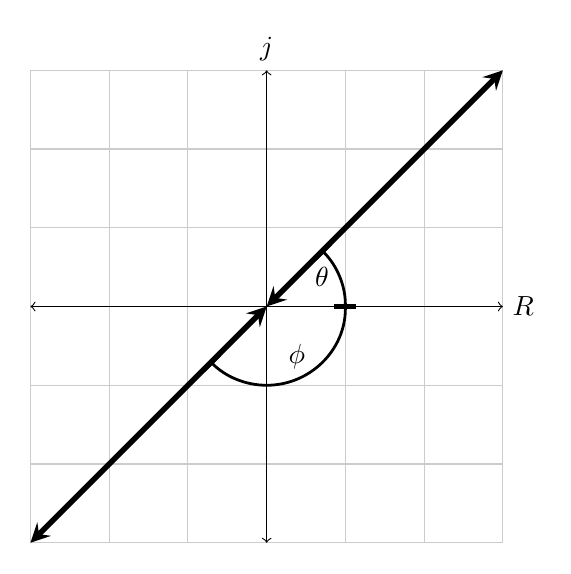
\begin{tikzpicture}
    \draw[thin,gray!40] (-3,-3) grid (3,3);
    \draw[<->] (-3,0)--(3,0) node[right] {$R$};
    \draw[<->] (0,-3)--(0,3) node[above]{$j$};
    
    \draw[line width=2pt,black,stealth-stealth] (-3,-3)--(0,0) ;
    \draw[line width=2pt,black,stealth-stealth] (0,0)--(3,3) ;
    \draw[line width=1pt,black,|-|] (1,0) arc (0:45:1) node [midway,left]{$\theta$};
    \draw[line width=1pt,black,|-|] (1,0) arc (0:-135:1) node [midway, above]{$\phi$};
\end{tikzpicture}
\caption*{Plano $z$}
    \end{minipage}
    \begin{minipage}{0.49\textwidth}
        \centering
        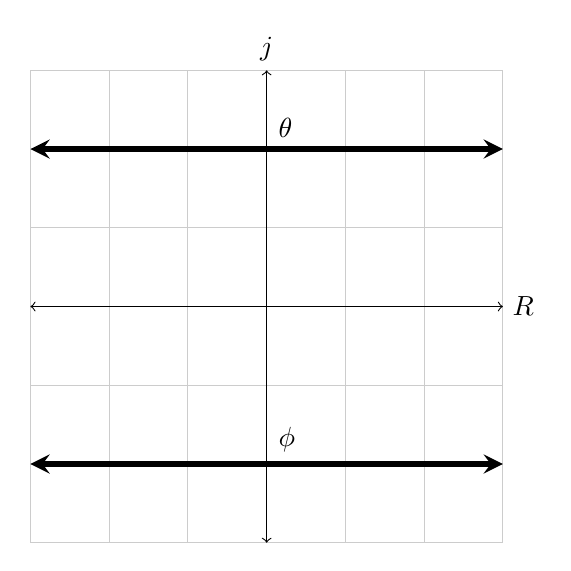
\begin{tikzpicture}
    \draw[thin,gray!40] (-3,-3) grid (3,3);
    \draw[<->] (-3,0)--(3,0) node[right] {$R$};
    \draw[<->] (0,-3)--(0,3) node[above]{$j$};
    
    \draw[line width=2pt,black,stealth-stealth] (-3,2)--(3,2)  node [midway,anchor=south west]{$\theta$};
    \draw[line width=2pt,black,stealth-stealth] (-3,-2)--(3,-2) node [midway,anchor=south west]{$\phi$};
\end{tikzpicture}
\caption*{Plano $w$}
    \end{minipage}
    \caption{}
    \label{fig:LnF1}
\end{figure}
El mapeo de las circunferencias y arcos es justo contrario al de rectas y semirrectas, al estar definidas por un modulo constante y un argumento variable serán mapeadas en lineas verticales.
\begin{equation}
   z_b=re^{j\theta}\begin{cases}
        r=\kappa\\
        a\leq\theta\leq b
   \end{cases} 
\end{equation}
Transformando:
\begin{equation}
    w_b=\ln{(z_b)}\lrah w_b=\ln{(r)}+j\theta\begin{cases}
        r=\kappa\\
        a\leq\theta\leq b
    \end{cases}
\end{equation}
Las lineas verticales en el plano $w$ que sean un mapeo de una circunferencia o un arco siempre estarán acotadas entre $\pi$ y $-\pi$ por como se define una circunferencia.
\begin{figure}[H]
    \centering
    \begin{minipage}{0.49\textwidth}
        \centering
        \begin{tikzpicture}
    \draw[thin,gray!40] (-3,-3) grid (3,3);
    \path[fill=vorange,fill opacity=0.6,even odd rule] (-3,-3) rectangle (3,3) (0,0) circle(1);
    \path[line width=2pt,black,dashed, fill=mlgb,fill opacity=0.6] (0,0) circle(1);
    
    \draw[<->] (-3,0)--(3,0) node[right] {$R$};
    \draw[<->] (0,-3)--(0,3) node[above]{$j$};
    \draw[line width=2pt,black,dashed] (0,0) circle(1);
    \draw[line width=1pt,black,|-|](0,0)--(1,0)node[midway,below]{$1$};
    \draw[line width=2pt,black,|-|] (0.7071*2,0.7071*2) arc(45:-45:2);
    \draw[line width=1pt,black,|-|](0,0)--(0.8192*2,0.5735*2)node[midway,above right,sloped]{$r$};
    
\end{tikzpicture}
\caption*{Plano $z$}
    \end{minipage}
    \begin{minipage}{0.49\textwidth}
        \centering
        \begin{tikzpicture}
    \draw[thin,gray!40] (-3,-3) grid (3,3);
    \path[fill=mlgb,fill opacity=0.6] (-3,-3) rectangle (0,3);
    \path[fill=vorange,fill opacity=0.6] (3,3) rectangle (0,-3);
    
    \draw[<->] (-3,0)--(3,0) node[right] {$R$};
    \draw[<->] (0,-3)node [anchor=south east]{$-\pi$}--(0,3) node[above]{$j$} node [anchor=north east]{$\pi$};
    \draw[line width=2pt,black,|-|] (1,-1.5)--(1,1.5) node[midway, anchor=south west]{$\ln{(r)}$};
    \draw[line width=2.5pt,black,dashed] (0,-3)--(0,3);

   
\end{tikzpicture}
\caption*{Plano $w$}
    \end{minipage}
    \caption{}
    \label{fig:LnF2}
\end{figure}
Para el caso de las lineas verticales y horizontales utilizaremos el mismo método que se utilizo para la función $z^{1/2}$.
Expresando las lineas en su forma polar:
\begin{equation}
    \begin{aligned}
        &z_a=\sqrt{\kappa_1^2+y^2}\hspace{0.2cm}e^{j\arctan{(y/\kappa_1)}}\\
        &\\
        &z_b=\sqrt{x^2+\kappa_2^2}\hspace{0.2cm}e^{j\frac{\arctan{(\kappa_2/x)}}{2}}
    \end{aligned}
\end{equation}
Aplicando la función $\ln{(z)}$ a $z_a$ obtenemos:
\begin{equation}
    w_a=\ln{(z_a)}\lrah w_a=\ln{(\sqrt{\kappa_1^2+y^2})}+j\arctan{(y/\kappa_1)}
\end{equation}
Entonces el mapeo estar dado por el siguiente sistema de ecuaciones:
\begin{equation}
    w_a\begin{cases}
        u=\ln{(\sqrt{\kappa_1^2+y^2})}
        v=\arctan{(y/\kappa_1)}
    \end{cases}
\end{equation}
Expresando $y$ en función de $v$:
\begin{equation}
    v=\arctan{(y/\kappa_1)}\lrah\tan{(v)}\cdot\kappa_1=y
\end{equation}
Y resolviendo por sustitución en $u$:
\begin{equation}
    \begin{aligned}
         u=\ln{(\sqrt{\kappa_1^2+y^2})}\lrah &u=\ln{(\sqrt{\kappa_1^2+(\tan{(v)}\cdot\kappa_1)^2})}\\
                                            &u=\ln{(\kappa_1\sqrt{1+\tan{(v)}^2})}\\
                                            &u=\ln{(\kappa_1)}+\ln{(\sqrt{1+\tan{(v)}^2})}
    \end{aligned}
\end{equation}
En el caso de las lineas horizontales el mapeo es igual a :
\begin{equation}
    u=\ln{(\kappa_2)}+\ln{(\sqrt{1+\frac{1}{\tan{(v)}^2}})}
\end{equation}
\begin{figure}[H]
    \centering
    \input{Plots/FuncionesComplejos/Mappeo/LogNa/LnCF}
    \caption*{}
    \label{fig:enter-label}
\end{figure}

\unsection{Función bilineal}
Una función bilineal es una conjunción de las funciones de desplazamiento, ampliación y reciproca y suele ser de la forma:
\begin{equation}
    w=\frac{a\cdot z+b}{c\cdot z+d}
    \label{eq:DefBil}
\end{equation}
Siendo $a$, $b$, $c$ y $d$ constantes.
Una función bilineal, al ser una construcción de otras funciones, se puede separar en distintas transformaciones.

Si realizamos una división de polinomios:
\begin{equation}
    \begin{array}{*1r @{\hskip\arraycolsep}c@{\hskip\arraycolsep} *{11}r}
        az+b &  &|\underline{cz+d}  \\
        -az-\frac{ad}{c}&        & \frac{a}{c}\\[5pt]
        \cline{1-1}
        b-\frac{ab}{c}    &          &    \\[-5pt]
\end{array}
\end{equation}
Entonces:
\begin{equation}
    az+b=\frac{a}{c}(cz+d)+(b-\frac{ab}{c})
    \label{eq:Bil1}
\end{equation}
Si remplazamos \ref{eq:Bil1} en \ref{eq:DefBil}
\begin{equation}
\begin{aligned}
    w=\frac{a\cdot z+b}{c\cdot z+d}\lrah W=&\cfrac{\frac{a}{c}(cz+d)+(b-\frac{ab}{c})}{c\cdot z+d}\\
                                          =&\cfrac{a}{c}+\cfrac{(b-\cfrac{ab}{c})}{c}\cdot\cfrac{1}{z+\frac{d}{c}}                          
\end{aligned}
\end{equation}
Al ser $a$, $b$, $c$ y $d$ constantes los términos $\frac{a}{c}$ y $\frac{d}{c}$ son desplazamientos por y el termino $\frac{(b-\frac{ab}{c})}{c}$ es una ampliación, asignando $z_0$, $z_1$ y $\kappa$ a cada uno de los términos obtenemos:
\begin{equation}
    w=z_0+\kappa\cfrac{1}{z+z_1}
\end{equation}
Entonces para computar el mapeo primero realizaremos el desplazamiento en $z_1$ luego seguiría la función reciproca, después la ampliación en $\kappa$ y por ultimo el desplazamiento en $z_0$.
Planteando una función bilineal cualquiera:
\begin{equation}
    f_{(z)}=\frac{3z+j2}{z}
\end{equation}
Podemos fácilmente separar los elementos que componen esta bilineal.
\begin{equation}
    f_{(z)}=3+2j\frac{1}{z}
\end{equation}
En este caso la ampliación conlleva también una rotación. Planteando un numero complejo en su forma exponencial para cubrir como se mapean circunferencias y rectas que pasen por el origen:
\begin{equation}
    w=3+2j\cfrac{1}{re^{j\theta}}\lrah 2=3+\frac{2}{r}e^{j(\pi-\theta)}
\end{equation}
En el caso que queramos representar un arco:
\begin{equation}
    z=re^{j\theta}\begin{cases}
        r=2\\
        -\frac{\pi}{3}\leq\theta\leq\frac{2\pi}{3}
    \end{cases}
\end{equation}
Este sera mapeado en otro arco de radio $r=1$, con centro en $(3,j0)$ y argumento de $\frac{\pi}{3}\leq\theta\leq\frac{4\pi}{3}$.
Casos en el que tengamos un desplazamiento en el numerador es recomendable plantearlo de manera gráfica, para luego realizar un análisis mas detallado,  por ejemplo sea una transformación bilineal de la forma:
\begin{equation}
    f_{(z)}=\cfrac{3z+2}{z+3}
\end{equation}
Realizando la división nos queda:
\begin{equation}
    w=\cfrac{3(z+3)-7}{z+3}\lrah w=3-7\cfrac{1}{z+3}
\end{equation}
Y queremos mapear una linea vertical que pase por el punto $(2,j0)$. Gráficamente podemos plantear 4 planos distintos en los cuales se apliquen las transformaciones de forma progresiva.
\begin{figure}[H]
    \centering
    \begin{tikzpicture}[node distance=4.5cm,thick,auto,main node/.style={rectangle,draw}]
    \node[main node] (1) {Plano $z$};
    \node[main node] (2) [below of=1] {Plano $\gamma$};
    \node[main node] (3) [right of=2] {Plano $\tau$};
    \node[main node] (4) [right of=3] {Plano $\lambda$};
    \node[main node] (5) [above of=4] {Plano $w$};
    \path[every node/.style={font=\sffamily\small}];
    \draw[-latex]
    (1) edge  node {Traslación $z_1$} (2)
        edge  node {$F_{(z)=}z_0+\kappa\cfrac{1}{z+z_1}$} (5)
    (2) edge  node {Reciproca $\frac{1}{z}$} (3)
    (3) edge  node {Escalado $\kappa$} (4)
    (4) edge  node[right] {Traslación $z_0$} (5);
\end{tikzpicture}
    \caption{Diagrama de flujo de una mapeo bilineal}
    \label{fig:DiagBil}
\end{figure}
La linea primero es desplazada por $z_1=3$, haciendo que ahora pase por el punto $(5,j0)$, sabiendo como se comporta la función reciproca de la ecuación \ref{eq:1/ZVer} sabemos que esta linea vertical sera transformada en una circunferencia de centro $(\frac{1}{10},j0)$ y de radio $r=\frac{1}{10}$, luego esta circunferencia es ampliada en un factor $\kappa=-7$ llevando el centro a $(-\frac{7}{10},j0)$  y el radio a $r=\frac{7}{10}$ y por ultimo un desplazamiento $z_0=3$ llevando el centro de la circunferencia a $(\frac{23}{10})$.
\begin{figure}[H]
    \centering
    \begin{minipage}{0.49\textwidth}
        \centering
        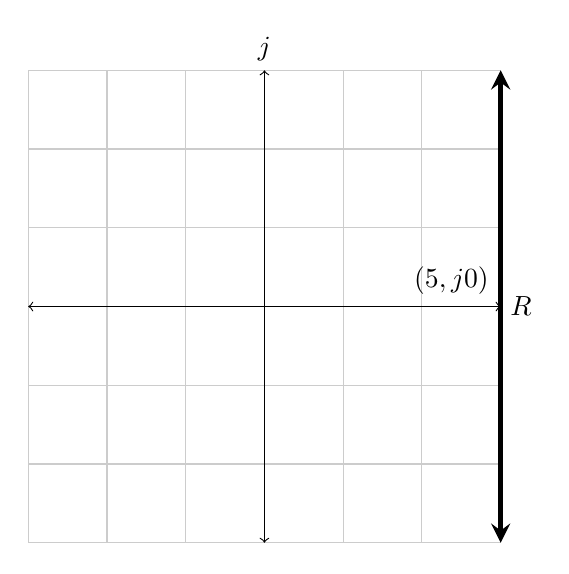
\begin{tikzpicture}
    \draw[thin,gray!40] (-3,-3) grid (3,3);
    \draw[<->] (-3,0)--(3,0) node[right] {$R$};
    \draw[<->] (0,-3)--(0,3) node[above]{$j$};
    \draw[line width=2pt, black,stealth-stealth] (3,-3)--(3,3) node[midway,anchor=south east]{$(5,j0)$};
    
\end{tikzpicture}
\caption*{Plano $\gamma$}
    \end{minipage}
    \begin{minipage}{0.49\textwidth}
        \centering
        \begin{tikzpicture}
    \draw[step=2.0,thin,gray!40] (-3,-3) grid (3,3);
    \draw[<->] (-3,0)--(3,0) node[right] {$R$};
    \draw[<->] (0,-3)--(0,3) node[above]{$j$};
    
    \draw[line width=2pt,black,-] (0.2,0) circle(0.2);
    
\end{tikzpicture}
\caption*{Plano $\tau$}
    \end{minipage}
    \begin{minipage}{0.49\textwidth}
        \centering
        \input{Plots/FuncionesComplejos/Mappeo/Bilineal/BilF3}
    \end{minipage}
    \begin{minipage}{0.49\textwidth}
        \centering
        \begin{tikzpicture}
    \draw[step=1.7,thin,gray!40] (-3,-3) grid (3,3);
    \draw[<->] (-3,0)--(3,0) node[right] {$R$};
    \draw[<->] (0,-3)--(0,3) node[above]{$j$};
    \draw[line width=2pt,black,-] (2.3,0) circle(0.7);

\end{tikzpicture}
\caption*{Plano $W$}
    \end{minipage}
    \caption{Aplicación método gráfico}
    \label{fig:TransBil}
\end{figure}

\unsection{Funciones como campos vectoriales}
Una función compleja se puede representar también como un campo vectorial, tomando una función cualquiera $f_{(x,jy)}=u+jv$ podemos representar la transformación del pano $z$ a través de vectores que tengan por punto de origen $(x,jy)$ y por punto final la suma entre el punto de origen y el punto transformado $w$ siendo esto igual a $(x+u,j(y+v))$.Para estas representaciones gráficas se separar la información en 2 gráficos distintos, un campo vectorial normalizado (quiere decir que a cada vector resultante se lo divide por su propia magnitud dejando un vector de modulo $=1$) solo útil para ver la dirección en la que se mapea el punto $(x,jy)$ y un campo escalar con el valor del modulo de los vectores, este ultimo se lo suele representar con colores o en un gráfico tridimensional siendo el eje $"z"$ representante de la magnitud del vector.

Un ejemplo seria el de la función $\frac{1}{z}$, de las secciones anteriores sabemos que a medida que el punto $(x,jy)$ este mas cercano al origen del plano $z$ mas lejos sera mapeado en el plano $w$ y viceversa. Tomemos el ejemplo del punto $(0.1,j0.1)$, pasándolo a su forma exponencial obtenemos $0.1414...e^{j\frac{\pi}{4}}$, y aplicando la función reciproca obtenemos el punto mapeado estará en $7.07e^{-j\frac{\pi}{4}}=(5,-j5)$. Entonces en la representación vectorial el vector asociado al punto $(0.1,j0.1)$ se extenderá desde el punto $(0.1,j0.1)$ al punto $(5.1,j-4.9)$ que normalizándolo seria $(0.721,-j0.65)$ y en el campo escalar en el punto $(0.1,j0.1)$ la ordenada a $z$ seria igual a $7.07$ que es el valor del modulo del vector sin normalizar.


\begin{figure}[H]
    \centering
    \begin{minipage}{0.49\textwidth}
        \centering
        %\input{Plots/FuncionesComplejos/VectFil/InvVectF1}
    \end{minipage}
    \begin{minipage}{0.49\textwidth}
        \centering
        %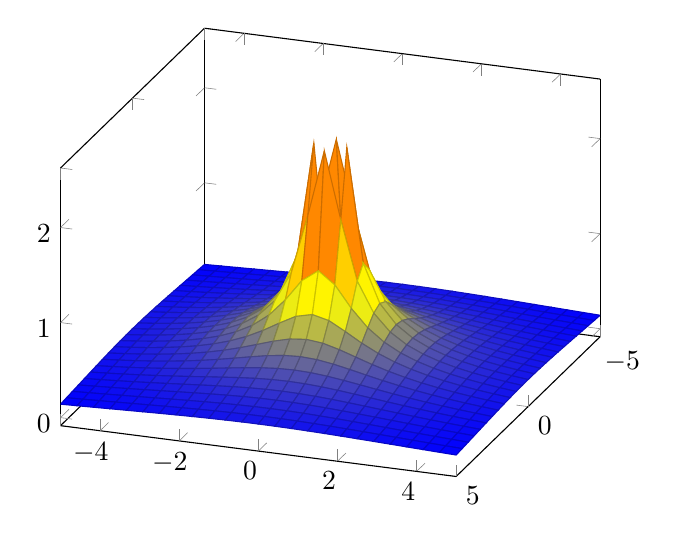
\begin{tikzpicture}
\begin{axis}[
 view={110}{30},
    unbounded coords=jump,
    z filter/.expression={
        z>20 ? nan : z
    }
]
\addplot3[surf,]{sqrt((-x/(x^2+y^2))^2+(y/(x^2+y^2))^2)};
\end{axis}
\end{tikzpicture}
\caption*{Campo escalar del modulo}
    \end{minipage}
    \caption{Representacion vectorial de la función $1/z$}
    \label{fig:VectFInvz}
\end{figure}
\begin{figure}[H]
    \centering
    \begin{minipage}{0.49\textwidth}
        \centering
        %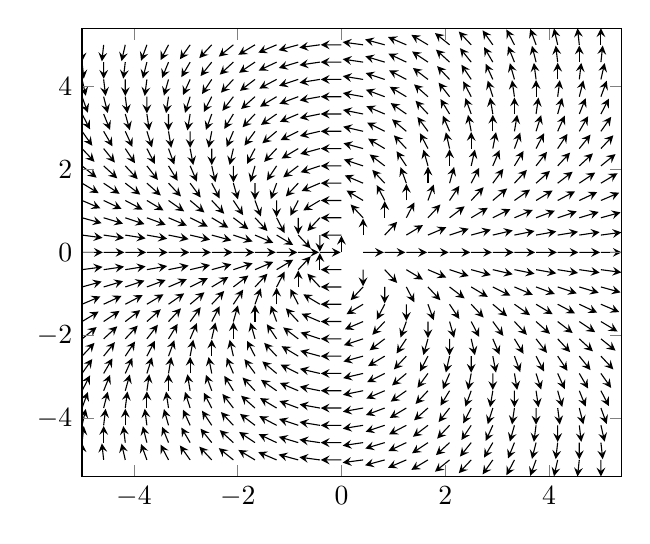
\begin{tikzpicture}
\begin{axis}[
view = {0}{90},
%unbounded coords=jump,
   % x filter/.expression={
   %     x>9 ? nan : x
   % },
%unbounded coords=jump,
  %  y filter/.expression={
   %     y>9 ? nan : y
  %  }
]
\addplot3[
        quiver = {
                u = {(x^2-y^2)/sqrt((x^2-y^2)^2+(2*x*y)^2)},
                v = {(2*x*y)/sqrt((x^2-y^2)^2+(2*x*y)^2)},
            scale arrows = 0.4},
            domain = -5:5,
            domain y = -5:5,
        -stealth] {0};
\end{axis}
\end{tikzpicture}
\caption*{Representación vectorial normalizada}
    \end{minipage}
    \begin{minipage}{0.49\textwidth}
        \centering
        %\input{Plots/FuncionesComplejos/VectFil/z^2EscF1}
    \end{minipage}
    \caption{Representacion vectorial de la función $z^2$}
    \label{fig:VectFZ^2}
\end{figure}
\unsubsection{Poly-vector field}
Si se aplica el operador de conjugación sobre las representaciones vectoriales de las funciones complejas se obtiene lo que se denomina un campo poly-vectorial que forman patrones de flujo en campos en los cuales existe una "singularidad":
\begin{figure}[H]
    \centering
    %\input{Plots/FuncionesComplejos/VectFil/InvPloyVect}
    \caption{Poly-vector field de la función 1/z}
    \label{inv-Poly-vector}
\end{figure}
\begin{figure}[H]
    \centering
    \input{Plots/FuncionesComplejos/VectFil/z^2PolyVect}
    \caption{Poly-vector field de la función 1/z}
    \label{z^2-Poly-vector}
\end{figure}